%%%%%%%%%%%%%%%%%%%%%%%%%%%%%%%%%%%%%%%%%%%%%%
%% Set up
%%%%%%%%%%%%%%%%%%%%%%%%%%%%%%%%%%%%%%%%%%%%%%
\documentclass{beamer}
\usepackage[utf8]{inputenc}
\usepackage[T1]{fontenc}
\usepackage{lmodern}
\usepackage{hyperref}
\usepackage{tikz}

\graphicspath{{../figure/}}

\AtBeginSection{\frame{\sectionpage}}
\addtocounter{framenumber}{-1}

%%%%%%%%%%%%%%%%%%%%%%%%%%%%%%%%%%%%%%%%%%%%%%
\title{Applying model-based geostatistical methods to analyse Celtic Sea survey
data}   
\author[shortname]{Paul Dolder, \inst{1} \and 
	James Thorson \inst{3} \and 
	Cóilín Minto\inst{1}}
\institute[shortinst]{\inst{1}Galway-Mayo Institute of Technology, Ireland \and
\inst{2} Centre for Environment, Fisheries and Aquaculture Science, UK \and
\inst{3} North West Fisheries Science Center, NOAA, USA}

\date{12 May, 2017} 
%%%%%%%%%%%%%%%%%%%%%%%%%%%%%%%%%%%%%%%%%%%%%%
\begin{document}
%%%%%%%%%%%%%%%%%%%%%%%%%%%%%%%%%%%%%%%%%%%%%%%
\frame{\titlepage} 
%\frame{\frametitle{Table of contents}\tableofcontents} 
%%%%%%%%%%%%%%%%%%%%%%%%%%%%%%%%%%%%%%%%%%%%%%%%
\section{Objectives} 
%%%%%%%%%%%%%%%%%%%%%%%%%%%%%%%%%%%%%%%%%%%%%%%%
\frame{\frametitle{Aim of analysis} 
\begin{enumerate}
\setlength\itemsep{2em}
\item Evaluate inter-species dynamics of main commercial fish populations in
	the Celtic Sea 
\item Explore strength of interdependence of fisheries on the different species
	(as an insight into the ability to spatially separate catches of
	species \textit{x} from species \textit{y})
\item Make efficient use of (and combine) the various surveys that have been
	undertaken in IE, FR, UK in past three decades.
\end{enumerate}
}

\frame{\frametitle{Expected outcomes}
\begin{enumerate}
\setlength\itemsep{2em}
	\item A useful index of abundance for the species/species groups
		following treatment for the irregular spatial survey coverage
		and sampling methods
	\item A measure of dependence of the different species in space and time.
	\item Insight into the spatio-temporal dynamics of the individual
		species as a pre-cursor to exploring how spatial abundance
		estimates can be used for fleet dynamics models.
\end{enumerate}
}

\frame{\frametitle{Where and what species-groups}
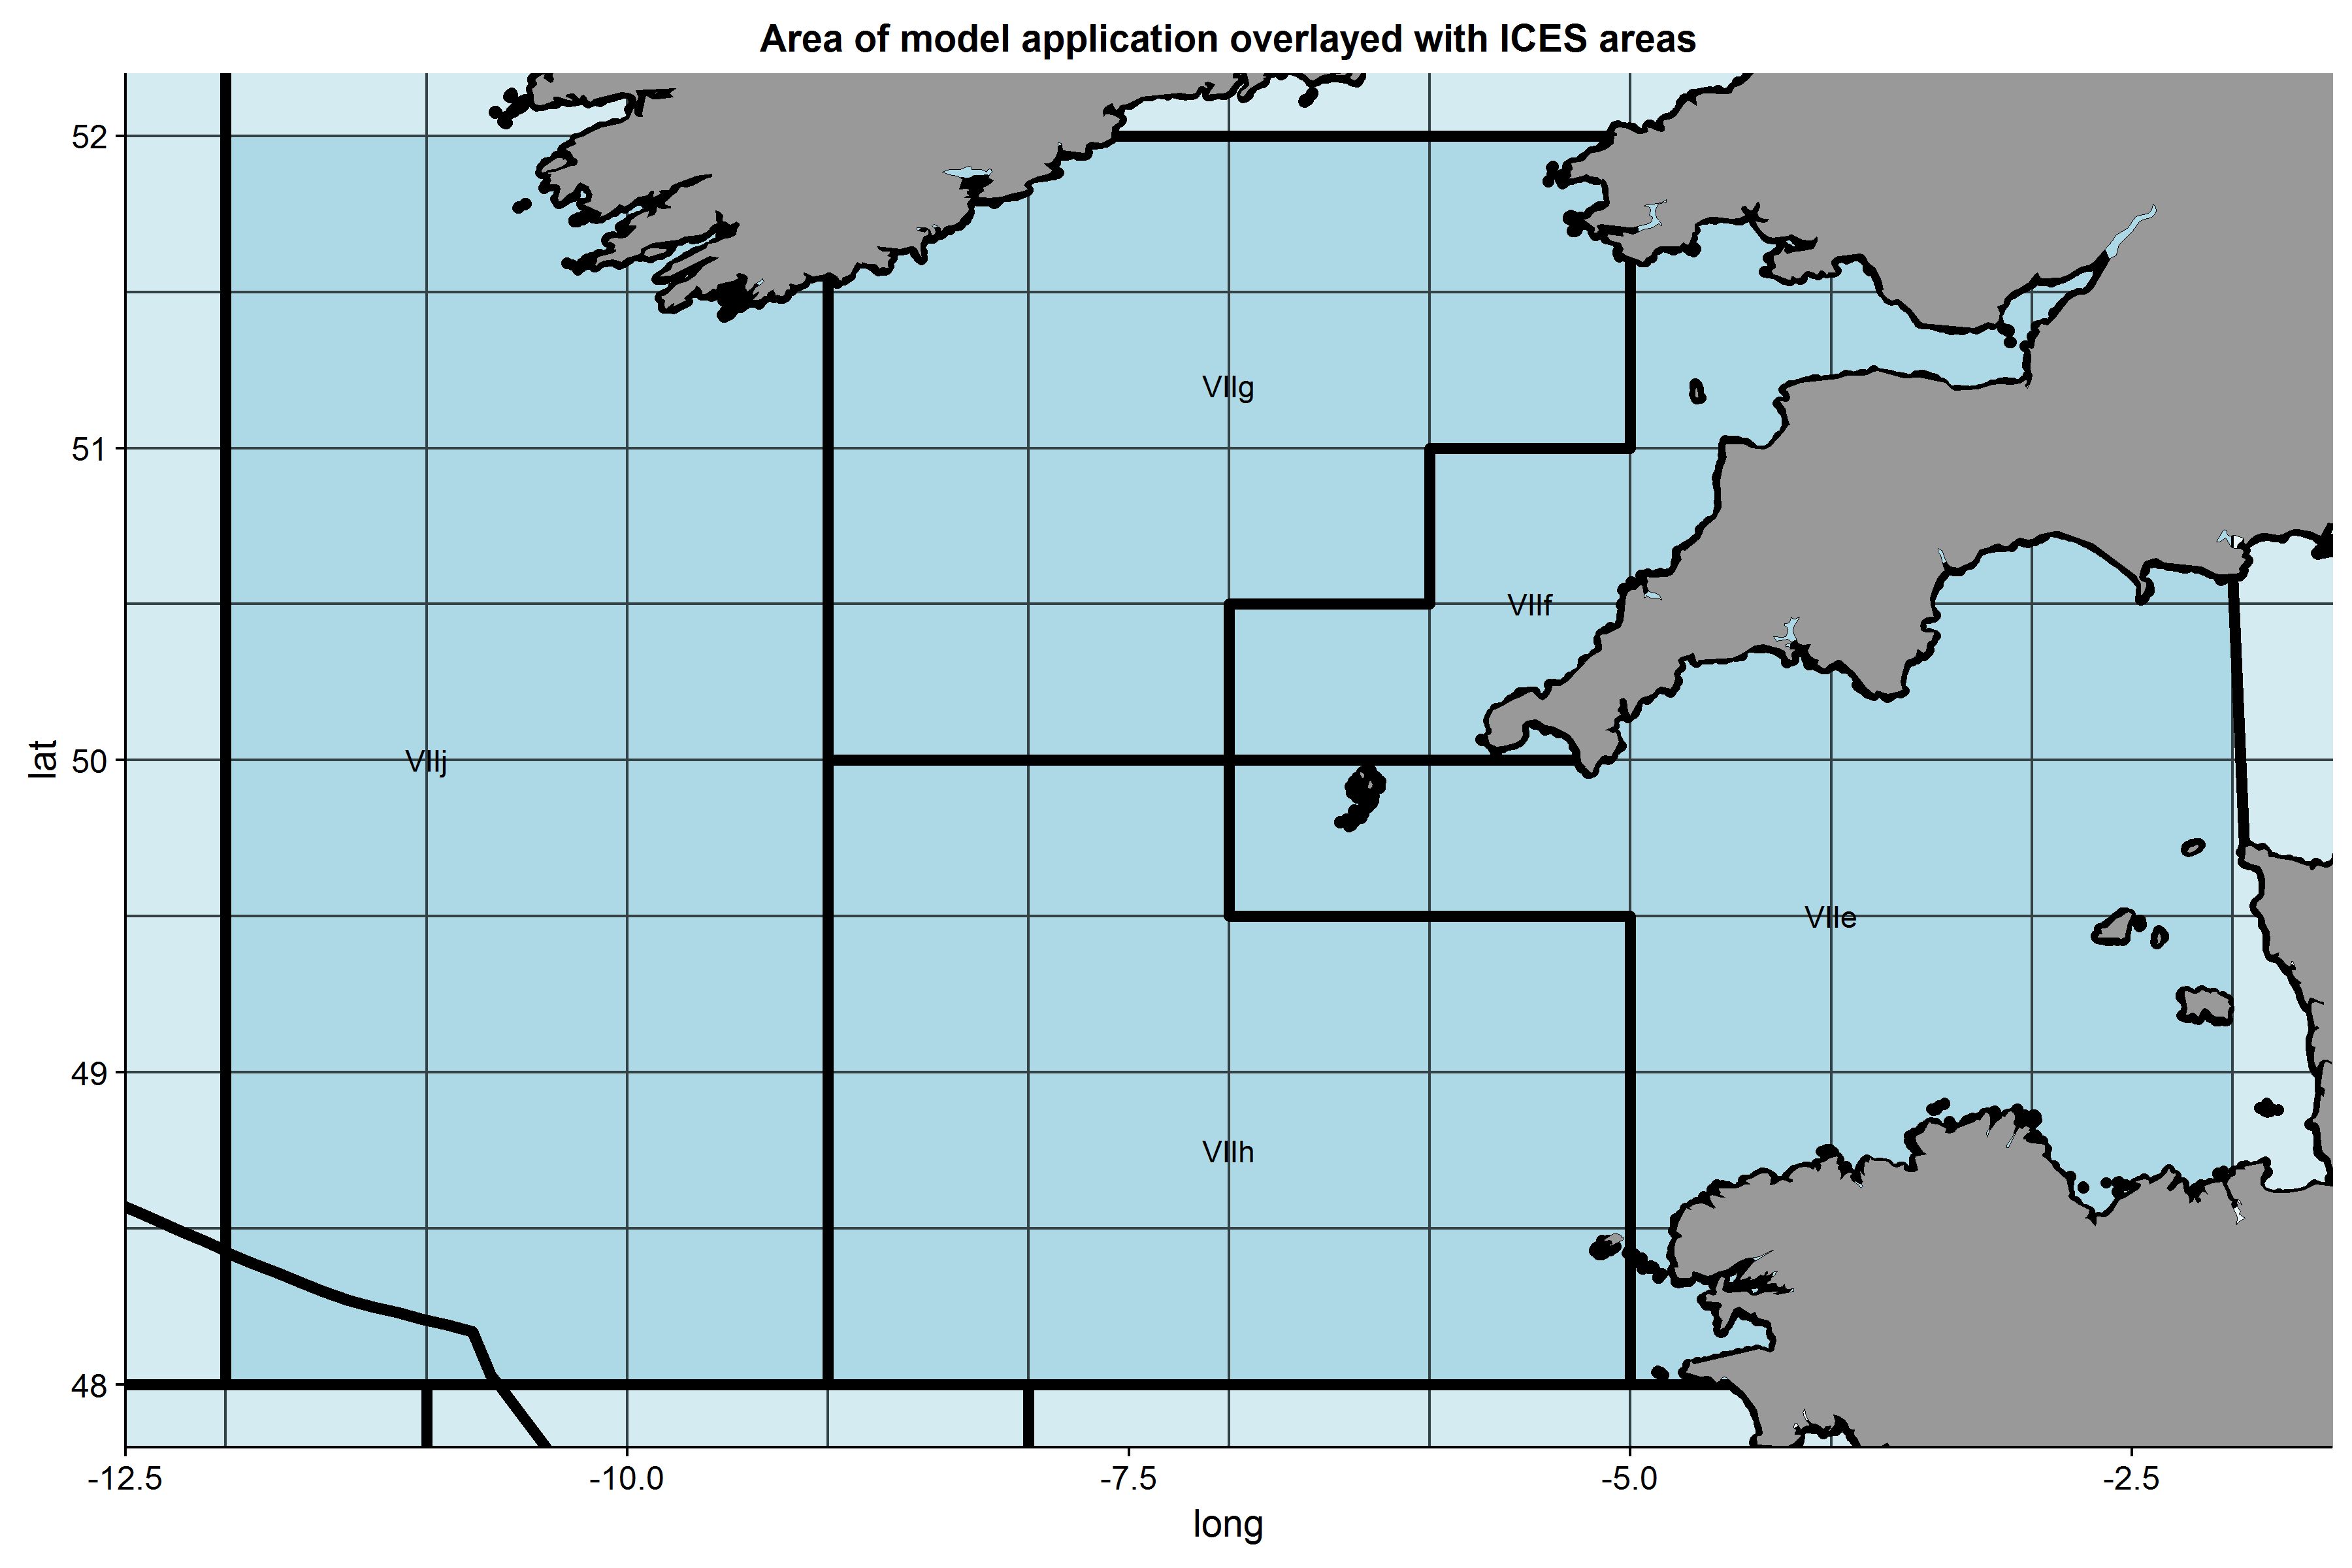
\includegraphics[width=0.5\linewidth]{AreaMap}

\begin{table}[!htb]
	\tiny
	\center
	\begin{tabular}{ p{1cm} p{2cm} p{3cm} p{1cm}}
		\hline
		Species code & Common name              & Species & MCRS (cm) \\
		\hline
		juv          & Juvenile                 & & \\
		adu          & Adult                    & & \\
		\hline
		bud          & Black bellied anglerfish & \textit{Lophius budgessa} & 32* \\
		cod          & Atlantic cod             & \textit{Gadus morhua} & 35 \\
		had          & Atlatic haddock          & \textit{Melanogrammus	aeglefinus} & 30 \\
		hke          & Atlantic hake            & \textit{Merluccius merluccius} & 27 \\
		meg          & Megrim                   & \textit{Lepidorhombus whiffiagonis} & 20\\
		pisc         & White bellied anglerfish & \textit{Lophius piscatorius} & 32* \\
		ple          & European Plaice          & \textit{Pleuronectes platessa} & 27 \\
		sol          & Common sole              & \textit{Solea solea} & 24 \\
		whg          & Atlantic whiting         & \textit{Merlangius merlangus} & 27 \\
		\hline
		\end{tabular}

\end{table}
}

\section{Methods}
\frame{\frametitle{Model overview}

\begin{itemize}
\small
		\setlength\itemsep{2em}
	\item VAST: Vector Autoregressive Spatial Temporal model
	\item Developed at the North West Fisheries Science Center, NOAA to
		incorporate methodological developments for species
		distributions and deriving standardised abundance indices in a
		mixed modelling framework. 
	\item Implements a delta-generalised linear mixed modelling (GLMM)
		framework that takes account of spatio-temporal correlations
		among multiple species / size classes 
	\item Spatio-temporal variation is represented through a
		three-dimensional Gaussian Random Field, based on a
		user-constructed mesh. 
	\item Full set of references in the working document and software
		available at \url{www.github.com/james-thorson/VAST}
\end{itemize}
	}


\frame{\frametitle{Model overview}

Four key components:

\begin{enumerate}
	\small
	\setlength\itemsep{2em}

	\item Joint Dynamic Species Distribution Model (JDSDM) able to take
		account of latent (unobserved) drivers which affect species
		distribution and density for one or more species, 
	\item separate modelling of encounter probability and positive catch
		rates (so called 'delta' and 'hurdle' models), 
	\item the use of Gaussian Markov Random Fields (GMRFs) to model the
		variation in probability of occurrence and density as a
		three-dimensional multivariate process (latitude, longitude and
		time) 
	\item set in a mixed modelling framework allowing the incorporation of
		both systematic (fixed) effects and random effects. 

\end{enumerate}

}

\frame{\frametitle{Methodology summary}

\begin{itemize}
	\small
	\setlength\itemsep{2em}

	\item Mesh construction: A spatial grid is constructed based on optimal
		clustering of the available point data using a k-means
		algorithm to provide \textit{n} knots representing the gaussian
		random fields used to derive spatial encounter probability and
		density estimates.

	\item  Associations among species / species-groups are modelled through
		implementing a factor analysis decomposition to define a
		function for each factor that returns a positive or negative
		association of one or more species with any location. Thus
		log-density of any species can then be described as a linear
		combination of factors:
		\begin{equation}
			\theta_{p}(s,t) = \sum_{j=1}^{n_{j}}
			L_{p,j}\psi_{j}(s,t) +\sum_{k=1}^{n_{k}}
			\gamma_{k,p}\chi_{k}(s,t)
		\end{equation}
	
\end{itemize}
}

\frame{\frametitle{Methodology summary}
	\begin{itemize}
	\setlength\itemsep{2em}
	\small

	\item Spatio-temporal encounter probability and positive catch rates
		are modelled separately with spatio-temporal encounter
		probability modelled using a logit-link linear predictor;
		\begin{equation}
			logit[p(s_{i},p_{i},t_{i})] = \gamma_{p}(p_{i},t_{i}) +
			\varepsilon_{p}(s_{i},p_{i},t_{i}) + \delta_{p}(p_{i},
			v_{i})
		\end{equation}

		and positive catch rates modelling using a gamma- distribution
		\begin{equation}
			gamma[r(s_{i},p_{i},t_{i})] = \gamma_{p}(p_{i},t_{i}) +
			\varepsilon_{p}(s_{i},p_{i},t_{i}) + \delta_{p}(p_{i},
			v_{i})
		\end{equation}

\end{itemize}
}
\frame{\frametitle{Methodology summary}
	\begin{itemize}
	\setlength\itemsep{2em}
	\small

	\item The spatio-temporal variation is modelled using a Gaussian
		Markov Random Field (GMRF) where catch data in nearby locations
		can be correlated, allowing inference about poorly sampled
		locations. 
	\item Specify a probability distribution for spatio-temporal
		variation in both encounter probability and positive catch rate, 
		$\varepsilon_{*}(s,p,t)$, with a three-dimensional multivariate 
		normal distribution so that:
		\begin{equation}
			vec[\mathbf{E}_{*}(t)] \sim MVN(0,\mathbf{R}_{*} \otimes
			\mathbf{V}_{{\varepsilon}{*}})
		\end{equation}
	\end{itemize}
	\centering
	\includegraphics[width=0.5\linewidth]{Matern}

	}

\frame{\frametitle{Methodology summary}
	\begin{itemize}
	\setlength\itemsep{2em}
	\small

	\item Vessels as either fixed or random effect, as well as predictive
		covariates (e.g. habitat quality, depth, temperature etc..) 
	\item Parameter estimation through Laplace approximation of the
		marginal likelihood using Template Model Builder (TMB).

	\item The index of abundance for species $p$ can then be derived from
		the summation of the spatio-temporal density estimates. 
		
		\begin{equation} I(p,t) =
			\sum_{s=1}^{n_{s}} a(s) \cdot
			logit^{-1}[\gamma_{p}(p,t) + \varepsilon_{p}(s,p,t)]
			\cdot exp[\gamma_{r}(p,t) + \varepsilon_{r}(s,p,t)]
		\end{equation}
\end{itemize}

}

\section{Data}

\frame{\frametitle{Survey data}
\begin{table}[!htb]
	\tiny
	\center
	\begin{tabular}{ p{1.5cm} p{3cm} p{2cm} p{1.5cm} }
		\hline
		Survey code    & Name 	& Gear & Temporal extent \\
		\hline
		CEXP / IE-IGFS & Celtic Explorer (IE)   & Otter trawl & 2003 - 2015 \\
		CARLHELMAR     & Carlhelmar (UK)	& Commercial beam trawl & 1989 - 2013 \\
		NWGFS          & North West groundfish survey (UK) & Beam trawl & 1988 - 2015 \\
		Q1SWBEAM       & Quarter 1 south-west beam trawl survey (UK) 	& beam trawl & 2006 - 2015 \\
		Q4SWIBTS       & Quarter 4 south-west international bottom trawl survey (UK) & Otter trawl & 2003 - 2010 \\
		THA2 / EVHOE    & EVHOE survey on Thalasa (FR) & Otter trawl & 1997 - 2015 \\
		WCGFS          & Wstern channel groundfish survey (UK) & Otter
		trawl (Portuguese high headline) & 1982 - 2004 \\
		\hline
	\end{tabular}
\end{table}
}

\frame{\frametitle{Survey data}
	\centering
\includegraphics[width=0.9\linewidth]{Survey_by_year-1}
}

\frame{\frametitle{Survey data}
	\centering
\includegraphics[width=0.9\linewidth]{Survey_effort_by_year-1}
}

\frame{\frametitle{Data processing (in the WD Annex)}
\begin{itemize}
	\setlength\itemsep{2em}
	\small
	\item Station and biological information was either downloaded from
		Datras or obtained directly from Cefas Fishing Survey System
		(FSS).
	\item Data were checked and cleaned for consistency (only valid hauls
		retained, outlier tow duration and distances removed,
		length measurements that were outliers were removed).
	\item Swept area per tow were estimated from the product of distance
		towed,  door spread (estimated through fitting a GAM so that:
		DoorSpread = s(Depth) + DoorWt + WarpLngth + WarpDiam +
		SweepLngth) and a gear and species-type specific correction
		factor.
	\item Length weight conversion factors were estimated from available
		data in Datras (EVHOE survey) and numbers at length were raised
		to weight per length class (based on a split between juveniles
		\textless MCRS and adults \textgreater MCRS).
\end{itemize}
}

\section{Model fitting and diagnostics}

\frame{\frametitle{Setup}

\begin{itemize}
	\setlength\itemsep{2em}
	\small
	\item The data was constrained to 1990 - 2015, reflecting the period
		during which the most spatially consistent data were available.
	\item The GMRF was set to 250 knots based on a compromise between
		spatial disaggregation and computational efficiency.
	\item The number of factors for the factor analysis decomposition set
		at nine (which explained \textgreater 95 \% of the variance in
		the encounter probability and density).
\end{itemize}

\begin{table}[!htb]
	\tiny
	\center
	\begin{tabular}{ p{1cm} p{2cm} p{2cm} p{1cm} p{1cm} }
		\hline
		Model & Catchability covariates & Density covariates & No Fixed
		effects & No Random effects \\
		\hline
		M0 & Vessel as Random effect & None  & 1462 & 129276 \\
		M1 & Vessel*Species group as fixed effect & None & 1674 & 129276   \\
		M2 & Vessel*Species group as fixed effect & Habitat and depth
		as fixed covariates & 1688 & 129276 \\ 
		\hline
	\end{tabular}
\end{table}
}

\frame{\frametitle{Spatial field}
	\centering
\includegraphics[width=0.5\linewidth]{SpatialDataAndKnots}

}

\frame{\frametitle{Q-Q plots}
	\centering
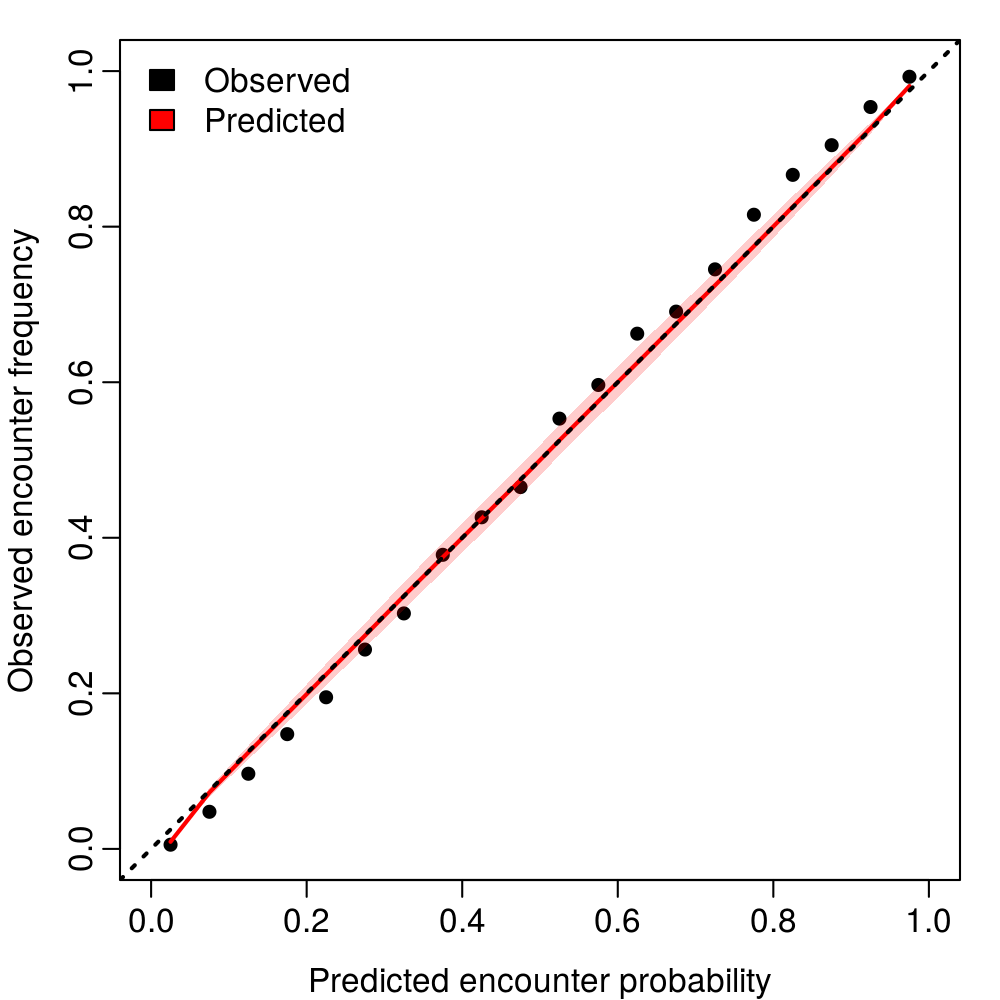
\includegraphics[width=0.47\linewidth]{Diag--Encounter_prob}
\includegraphics[width=0.5\linewidth]{Q-Q_plot}

}

\frame{\frametitle{Spatial correlation}
	\centering
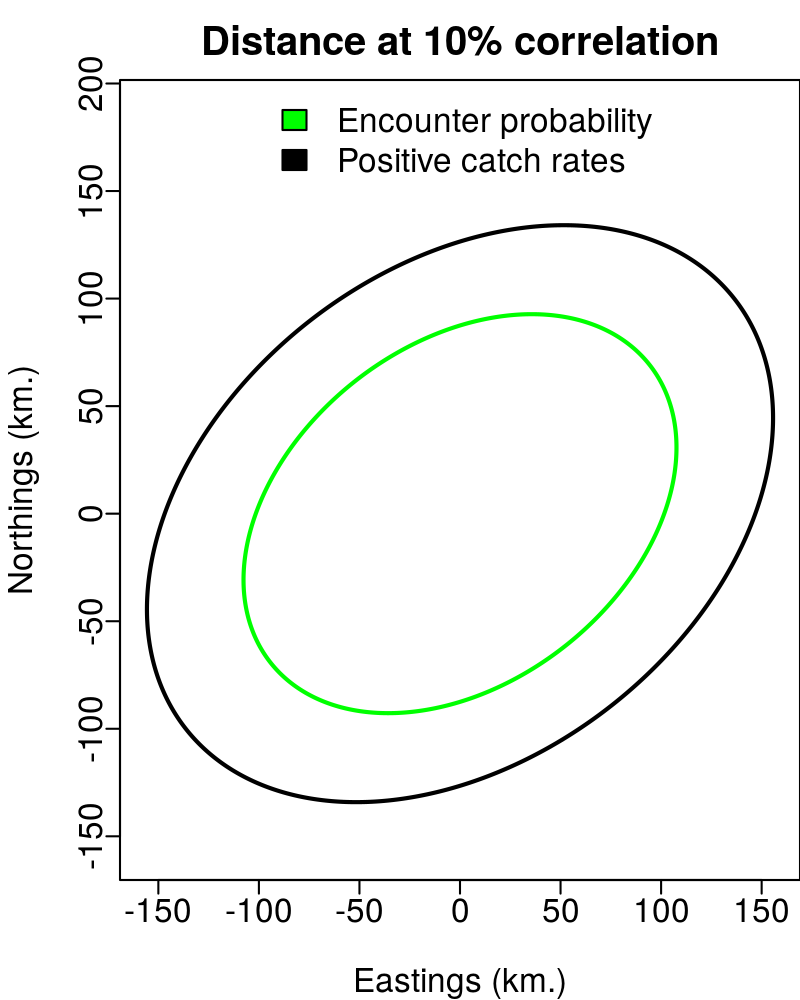
\includegraphics[width=0.5\linewidth]{Aniso}
}

\section{Parameter estimates}

\frame{\frametitle{Catchability parameters}

	Switch to the WD 
}

\frame{\frametitle{Factor maps - average spatial encounter prob}
	\centering
\includegraphics[width=0.9\linewidth]{Factor_maps--Omega1}

}

\frame{\frametitle{Factor loading - spatio-temporal density}
	\centering
\includegraphics[width=0.9\linewidth]{Factor_loadings--Epsilon2}

}

\frame{\frametitle{Species correlations}
	\centering
\includegraphics[width=0.8\linewidth]{Spatio-temporal_Covariances--Analytic}
}

\section{Global and spatial indices}

\frame{\frametitle{Global indices}
	\centering
\includegraphics[width=0.95\linewidth]{IndexGGplot}

}

\frame{\frametitle{Relative Indices Vs Assessment SSB}
	\centering
\includegraphics[width=0.8\linewidth]{RelativeIndexVRelativeAssessSSB}

}

\frame{\frametitle{Adult cod spatial densities}
	\centering
\includegraphics[width=0.95\linewidth]{"Field_Dens--Gadus morhua_Adu"}

}

\frame{\frametitle{Juvenile cod spatial densities}
	\centering
\includegraphics[width=0.95\linewidth]{"Field_Dens--Gadus morhua_Juv"}

}

\frame{\frametitle{Adult plaice spatial densities}
	\centering
\includegraphics[width=0.95\linewidth]{"Field_Dens--Pleuronectes platessa_Adu"}

}

\frame{\frametitle{Juvenile plaice spatial densities}
	\centering
	\includegraphics[width=0.95\linewidth]{"Field_Dens--Pleuronectes platessa_Juv"}
}

\frame{\frametitle{Summary}

	\begin{itemize}
	\setlength\itemsep{2em}
	\small
\item VAST provides a fully model-based geo statistical method incorporating spatial
and temporal correlations within and across species and taking account of
differences in survey design. 

\item As expected, strong correlations within groups (gadoids, flats, shelf)
	indicates may be spatially difficult to separate in mixed fisheries. \\

\item The derived indices show good agreement with assessment outputs and offer a
potential method to standardise across the various surveys - 
\begin{itemize}
\item may be useful for producing indices with longer time series than used at
	present and may be extended to data poor stocks currently without
	indices. 
\item Another potential use could be as a useful tool to identify spatial gaps
	(e.g. look at CVs of density estimates spatially) or the consequences
	of removing survey stations or surveys and what impact that might have
	on indices.

\end{itemize}
\end{itemize}

}

\frame{\frametitle{Acknowledgements}
	\begin{itemize}
	\setlength\itemsep{2em}
	\small
		\item Jim \& others at NOAA and the University of Washington
			for hosting me 
		\item  Colm, Hans, Dave, Ian, Stephen, Chris, Lisa, Tim for
			discussions on the data and preliminary outputs
		\item Irish Centre for High End Computing (ICHEC;
			\url{www.ichec.ie}) for use of cluster computing
			facilities
		\item EU MARES (\url{www.mares-eu.org}) Joint-doctoral programme
			on ecosystem health and conservation and Cefas Seedcorn
			for funding 
	\end{itemize}

}


%%%%%%%%%%%%%%%%%%%%%%%%%%%%%%%%%%%%%%%%%%%%%%%%
%%%%%%%%%%%%%%%%%%%%%%%%%%%%%%%%%%%%%%%%%%%%%%%%
\end{document}
%%%%%%%%%%%%%%%%%%%%%%%%%%%%%%%%%%%%%%%%%%%%%%%%
